\documentclass[10pt,a4paper]{report}
\usepackage[utf8]{inputenc}
\usepackage[english]{babel}
\usepackage{amsmath}
\usepackage{amsfonts}
\usepackage{amssymb}
\usepackage{color}
\usepackage{graphicx}
\author{A.M. Ahsan Feroz \\
\texttt{abdullah.feroz@aalto.fi}
\and
Md. Mohsin Ali Khan \\
\texttt{md.m.khan@aalto.fi}
\and
Elena Oat\\
\texttt{elena.oat@aalto.fi}
\and
Hasan M. A. Islam \\
\texttt{hasan.islam@aalto.fi}
\and
Md. Mesbahul Islam\\
\texttt{mdislam@cs.helsinki.fi} \\
\and
Tutor: Antero Juntunen
}
\title{T-110.5130 Mobile Systems Programming Final Report}
\begin{document}
\maketitle

\tableofcontents

\chapter{Introduction}
 

Now-a-days, people are so busy with their daily activities and hence, it is more likely for one to forget a schedule that might be very important. In the present hi tech world, mobile phones could be a great medium to keep track of the all the things and notify the user in the right time to perform a task. We have developed a $'$Task Manager$'$ which is initially named as $'$AndroTaskScheduler$'$. The very first version of our Android Task Scheduler will be a typical one which would be able to maintain and keep track of all of our schedules of every moment. The user can give temporal input to our application and the app will be responsible to remind the user by means of alarm about the temporal events. The application will always be running in the background and the reminder will pop up in a small screen at the desired time. The application will also have a view screen which can be used as an widget in the desktop with the list of tasks. The main motivation behind choosing Android platform are the followings:

 \begin{itemize}
   \item Android is the most widely used platform for mobile respecting the number of users and number of applications.
   \item Android app developers use the classic open source Linux OS. Any open source provides help for users to access its source code transparently and is available to any developer who wants to modify it or see how it works.
   \item Google provides all Android developers with an open source software development kit for the Android OS. They can create applications for Android and then test them on an Android simulator before loading them onto an actual Droid phone.
   \item The future of the Android platform looks bright for Android application developers who love to have access to everything. We can expect to see some interesting innovations both from Google and from the public as Android gains popularity.
 \end{itemize}

\section{Report Outline}

Chapter 1 will evaluate the results of our implementation with prospective development ideas and list of all challenging technologies we used in our app. Summary of used resources, quality metrics, software size etc., will be outlined in chapter 2 with some analysis compared to standard Google Calendar. Work practices and tools, and preliminary business model will be explained in chapter 3 and 4 respectively.

 
%-------------------------------------------------%
\chapter{Evaluation of the Results}
\label{results}

\section{What was our goal?}
The primary goal of the project was to learn how to develop a mobile application for Android platform. The scope of the project was to develop an application that provides the user functionality to do the following activities:

\begin{description}
 \item 1. View Existing Events
  \begin{itemize}
    \item Day view
    \item Week view
    \item Month view
  \end{itemize}
  
  \item 2. Create New Events
  \item 3. Edit Existing Events
  \item 4. Alarm and Bar notifications of the Events at the due time
\end{description}

\begin{figure}[h!]
\begin{center}
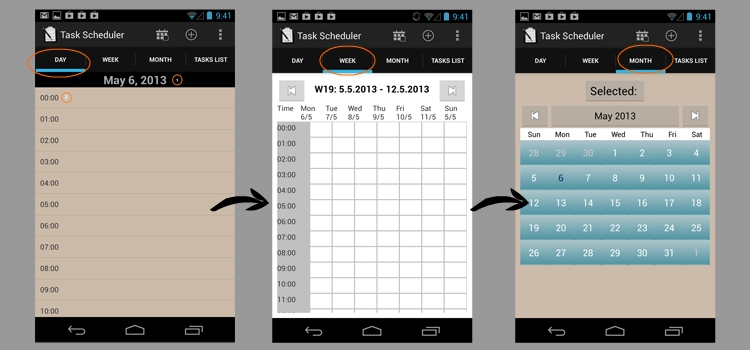
\includegraphics[scale=.5]{daymonthweek.jpg}  
\end{center}
\caption{Day, Week and Month View}
\label{hd}
\end{figure}


\section{Results}
\label{sresults}





\subsection{Day view}
When user will click an empty cell on day view layout, it will redirected to create new task activity if the cell is empty. Otherwise, it will redirect to edit task activity.




\subsection{Week view}

This view gives a snapshot of tasks of one week.

\begin{itemize}

 \item[$\bullet$] Initially the week view is loaded with current week days. There are two buttons, \textbf{\texttt{$'$prev$'$}} and \textbf{\texttt{$'$next$'$}}, for navigating to previous or next weeks respectively.
 \item[$\bullet$] The week days are partitioned into 24 hours. So, there are 168 (24*7) 'Cell's in this view. Each cell points an specific hour of a day. If there are saved tasks which are created for these week days then the corresponding cells are marked 'Green' when created.
 \item[$\bullet$] Each cell has two modes, \textbf{\texttt{$'$Selection$'$}} and \textbf{\texttt{$'$Navigation$'$}}. When a user touch a \textbf{\texttt{$'$Cell$'$}} first time, it will be in \textbf{\texttt{$'$Selection$'$}} mode. The cell will be in \textbf{\texttt{$'$Navigation$'$}} mode when same cell is touched again. If the Cell is empty then it will navigate to addNewTask view. Otherwise a dialog will pop-up with associated saved task data and there will be three buttons \textbf{\texttt{Edit, Delete and Cancel}}.
  
\end{itemize}
 

\subsection{Month view}

This view presents a month layout.

\begin{itemize}
  \item[$\bullet$] Initially this view shows current month. A user can navigate to next or previous months through \textbf{\texttt{$'$next$'$}} and \textbf{\texttt{$'$prev$'$}} image buttons.
  \item[$\bullet$] If user selects a date in the month view then the selection will redirect to corresponding Day View.
\end{itemize}

\subsection{Preference Settings}
 Our application includes settings that allow users to modify app features and behaviors. For example, some apps allow users to specify preferences e.g., notificationB4, notificationFreq, notificationType. \\




\begin{figure}[h!]
\begin{center}
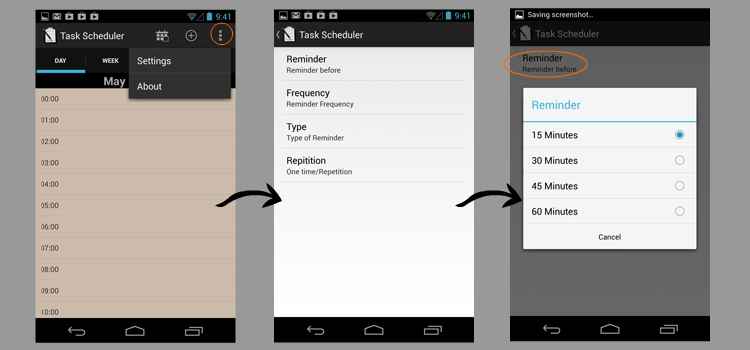
\includegraphics[scale=0.5]{settings.jpg}  
\end{center}
\caption{Preference Settings}
\label{hd}
\end{figure}

\subsection{Action Bar}

Action bar with Navigation has been implemented implemented with the following features:
\begin{itemize}

 \item[$\bullet$] Action bar \texttt{MODE} is TAB navigation. There are four \texttt{TABS}. Among these, three \texttt{TABS} are responsible for three different views and the fourth \texttt{TAB} is responsible for showing all saved data.
\item[$\bullet$] There is a menu on top right corner, which includes \texttt{Settings} and \texttt{About}. Users can set own preferences through \texttt{Settings} that include the followings:

	\begin{itemize}
	   \item[$\bullet$] Reminder.
	   \item[$\bullet$] Notification Before
	   \item[$\bullet$] Repetition
	   \item[$\bullet$] Type of Reminder
	\end{itemize}

\end{itemize}

\subsection{Database}

The application uses an sqlite database to store information about all the tasks created by the user and to store some default values of some global properties of the application. To store these information, it maintains to database table and number of methods in the DatabaseAdapter classs to do operation on these two tables.

Name of the two database tables are:

	\begin{itemize}
	  \item[$\bullet$]  master$\_$event  (To store all the events)
	  \item[$\bullet$]  global$\_$config to store all the default values of the global properties of the application e.g., notificationB4, notificationFreq, notificationType. Whenever a new event is created, the values specified in this table for these properties will be used to create the new event, unless the user explicitly mention the value of this properties.
	\end{itemize}
	
 \subsection{Service Granularity in Database}

   To integrate the above mentioned functionalities of our app at the front end with the database tables, it was required to implement some interface between front end and the database. The interface includes the following basic primitive services:
   \begin{itemize}
   	  \item createEvent
      \item deleteEvent
      \item editEvent
      \item getEventByDate
      \item getEventByID
      \item $\cdots$
      \item $\cdots$
      \item etc.
   \end{itemize}
  \begin{description}
  
   
  \item[\texttt{createEvent}] method is responsible for inserting task into database. Its processing details are as follows: 
   
   \begin{itemize}
     \item  If the \texttt{recurrenceFlag} parameter received from front end is null, it inserts a new row in the \texttt{master$\_$event} table using all the other given inputs. The \texttt{id} column is automatically populated by the database. In this case the \texttt{parentID} column of this table is populated as \texttt{0}.

\item If the \texttt{recurrenceFlag} is not null i.e., daily or weekly or monthly, it checks the \texttt{eventEndDayTime} and find/calculate all the child events and insert one row as parent event for the first occurrence and one row for each child event.

In this case, it populates the \texttt{parentID} column of the parent event as 0 The value of \texttt{parentID} column of the child events are populated with the value of the id column of the parent event.
   \end{itemize}
   
 \item[\texttt{deleteEvent}] deletes all the rows from the \texttt{master$\_$event} table which has the value id(received as input) in their id column or in their \texttt{parentID}.   
   
    \item[\texttt{editEvent}] takes the help of \texttt{createEvent} to edit a task. 
  \begin{itemize}
   
   \item If the received event to be edited is a single event or a parent event of a recurrent event, it deletes the event by calling the \texttt{deleteEvent} method and create a new Event by calling the \texttt{createEvent} method

	\item If the received event to be edited is a child event of a recurrent event, then it deletes the event by calling the \texttt{deleteEvent} method and then create a new Event by calling the createEvent method. While calling the create event method,it sets the recurrence flag to null and sets the editparentID variable to the ID of its \texttt{parentID}. This \texttt{editParentID} ensures that the edited child event still remains as the child of its parent.
   
     
\end{itemize}
   
 \end{description}  
	
 \section{Prospective Development Ideas}
	
 \section{Challenging Technologies}
 List of all challenging technological and environment related aspects of our app will be briefly outlined in this section.
  \subsection{SQLiteDatabase}
  
  \begin{description}
  
  
  
\item[Trouble with properly setting up SQLiteDatabase] At the beginning of our database implementations we frequently face error like as follows:

\begin{verbatim}
ERROR/Database(234): Leak found
ERROR/Database(234): Caused by: java.lang.IllegalStateException:
                 SQLiteDatabase created and never closed
ERROR/Cursor(31526): Finalizing a Cursor that has not been 
deactivated or closed.....
ERROR/Cursor(31526): android.database.sqlite.
DatabaseObjectNotClosedException: Application did not close 
the cursor or database object t
hat was opened here                  
\end{verbatim}

We come to realize that this exception is thrown when we have opened more SQLiteDatabase instances than we have closed. Same thing is also true for \texttt{Cursor} which is used for retrieving data from database. Managing the database can be complicated when first starting out with Android development, especially to those who are just beginning to understand the Activity lifecycle. Our learning is that the easiest solution is to make database instance a singleton instance across the entire application's lifecycle. This will ensure that no leaks occur, and will make your life a lot easier since it eliminates the possibility of forgetting to close your database as you code. Our application uses \texttt{DatabaseAdapter class} for the whole application.

The approach we used for the Singleton Database is that we have created an Abstract Factory to instantiate the SQLiteOpenHelper.

\item[Relief Using ADB shell]  ADB shell will work only after application will have been launched into our device or Emulator.
 
 \begin{verbatim}
 

hasan@eliteworm:~$ cd android-sdk-linux/platform-tools/
hasan@eliteworm:~/android-sdk-linux/platform-tools$ ./adb shell
# 
# cd /data/data/com.taskmanager/databases
#
# ls
taskManager.db
# 
# sqlite3 taskManager.db
SQLite version 3.6.22
Enter ".help" for instructions
Enter SQL statements terminated with a ";"
sqlite> 
sqlite> .schema

CREATE TABLE android_metadata (locale TEXT);
CREATE TABLE global_config(property TEXT PRIMARY KEY, valueType TEXT,
 textValue TEXT, intergerValue TEXT, dateValue TEXT);

CREATE TABLE master_event(id INTEGER PRIMARY KEY AUTOINCREMENT, 
recurrenceFlag TEXT, recurrenceEndDate TEXT, parentID TEXT, name TEXT, 
description TEXT, createTime TEXT, dueDate TEXT, notificationB4 TEXT, 
notificationFreq TEXT, notificationType TEXT);

sqlite> 
sqlite> select * from global_config;
NotificationB4|int||Fifteen|
NotificationFreq|int||Five|
NotificationType|text|Both|Five|
sqlite> 


 \end{verbatim}
 
 When we came to familiar with the checking our app databases using ADB shell, it helped us a lot to check the queries there and finally put that into our code. We can remove database, insert, update and remove data from database through ADB shell. All kinds of experiments with the database can be performed through ADB.


\end{description}

\subsection{Layout}

\subsection{Preference Settings}

We have used Android's \texttt{Preference APIs} to build an interface that is consistent with the user experience in other Android apps (including the system settings). Each \texttt{Preference} appears as an item in a list and provides the appropriate UI for users to modify the setting. \\

Our app requires to store the changes in preferences. For this, we had to use \texttt{SharedPreferences}. Each Preference you add has a corresponding key-value pair that the system uses to save the setting in a default \texttt{SharedPreferences} file for your app's settings. When the user changes a setting, the system updates the corresponding value in the \texttt{SharedPreferences} file. Apps need to directly interact with the associated \texttt{SharedPreferences} file is when it requires to read the value in order to determine your app's behavior based on the user's setting. \\


In order to make use of the preferences framework, the first step is to extend the \texttt{PreferenceActivity} class. This is just a convenience class that derives from \texttt{ListActivity} and allows to bootstrap the preferences \texttt{UI} from an \texttt{XML} file. Additionally, it automatically saves to \texttt{SharedPreferences} behind the scenes. Note that \texttt{SharedPreferences} is the interface responsible for accessing and modifying preference data and that we can manually manipulate it by calling the \texttt{getSharedPreferences} method of an Activity. In order to tie together our \texttt{PreferenceActivity} class and the \texttt{XML} layout file, we use the \texttt{addPreferencesFromResource} method. 

\subsection{Alarm Manager}

Prior to a set time of the start time of an event/task, the application notifies the user with an alarm. The user can set this prior time while creating an event/task. Otherwise the prior time will be set from the default settings of the application. When the alarm is generated, a new activity with a lay out is loaded and the default alarm ring tone of the application starts to play. In the lay out there is a button named “Notified”. When user taps this button, the phone gets back to the context where it was and the audio stops to play. \\


The default AlarmManager class has been used to implement this functionality. Whenever an alarm is created in the database, a Peding Intent is created. This Pending Intent is created with a normal intent the that fires an activity. The activity loads the Alarm layout and plays the default ring tone. Then the Pending Intent is sent to the android system through the AlarmManager to be executed at the specified time. \\


The Pending Intent remains in the system even if the application is not running and loads the activity when the specified time comes. It also does the same even if the phone is switched off. 

\subsection{Application Navigation}

ActionBar is a nice feature of Android which provides user actions and smooth navigation of an application. At the beginning of this application development we used only Activities and buttons to navigate between activities. But later we realized that ActionBar provides the navigation feature in a more smart way. It improves the UI also. But ActionBar works for API level 11 and above. So, we have to take decision for target devices and we agreed to work with ActionBar. We have also implemented 'Option Menu' for general 'Settings' and 'Action Items' to give users immediate action for specific situation. For example, 'Save' or 'Cancel' action item while creating new task or 'Edit' and 'Delete' action items in Day View.

The challenges we faced includes working with FragmentTransactions as we need to navigate and communicate between Tab fragments. Moreover we had to save the state of a TAB when a TAB is selected or re-selected.

\subsection{XML Layouts}

We experimented different types of layout in our application. Most of the XML uses Linear layout. We have avoided more complex and nested layouts in our application. If the nested level is high then it will be a performance issue and the application will take time to render the view.

In Day View we used List View to show the hour slots of a Day. The Week View and Month View are created dynamically at the run time of the application.

\subsection{Screen Orientation}

The activity actually stops and restarts every time the device orientation changes. To save the state of the application, Android calls the \texttt{OnSaveInstanceState(Bu- ndle bundle)} method before it destroys the Activity. The bundle object is passed in the \texttt{OnSaveInstanceState() callback} method to save small amount of data. Bundle is not designed to handle large amount of data. Restoring the saved state is done with the \texttt{onCreate() or onRestoreInstanceState ()} method.

We can also handle screen orientation by the following way:
\begin{itemize}
 \item In  Activity's manifest node we need to add: 
  \begin{verbatim}
 		android:configChanges="keyboardHidden|orientation"
   \end{verbatim}
   
  \item  Then within the Activity override the \texttt{onConfigurationChanged} method and call \texttt{setContentView} to force the GUI layout to be re-done in the new orientation.
  \begin{verbatim}
	  @Override
 	  public void onConfigurationChanged(Configuration newConfig) {
	  super.onConfigurationChanged(newConfig);
  	  setContentView(R.layout.myLayout);
	}
 \end{verbatim}
\end{itemize}

\subsection{NotificationManager}
A notification is a message that is required to notify user outside of our application's normal UI. We need to set a timestamp to tell the system to issue a notification, it first appears as an icon in the notification area. Our application notify the user about task schedule through status bar notification and alarm manager. 
 

 


%-------------------------------------------------%
\chapter{Metrics}

\section{Used Resources}

We have implemented our project in Eclipse and tested with Samsung phone and Tablet, HTC mobile phone and Emulator. Some of our team members build application in windows operating system and some in Unix operating system. \\

Every group member has an account on \texttt{Github}. A repository was created, which serves as a place for common development. All commits are accompanied by a message which states what changes have been made to the previous version.

\section{Quality Metrics}

\begin{itemize}
 \item User friendly
 \item Error density
 \item Robustness
 \item Liveness
 \item Application Security
\end{itemize}

\section{Software Size}

Total lines of Java source code are approx. 3500. \textit{\color{red}(Please mention the application size in terms of Kbytes here. also mention how much memory space it needs to create a task.)}

\section{Analysis}

We have compared our application with google calendar.\\

In google calendar user can create an event/task. Our application can do the same.
Prior to a time the google calendar notifies the user through mail, our application generates an alarm with the phone's default ring tone \\

In google calendar user can create a repeated event based on the day's of a week. For example, every Monday, Or every Tuesday or On Every Monday and Friday. In our application user can create repeated events based on the daily, weekly, monthly recurrence \\

In google calendar user can edit or delete an existing event. In our application user can do the same\\

In google calendar whenever the user edits the occurrence of a repeated event, it asks the user about editing only that particular event or the whole series. In our application, when the user edits the child event, only that event is edited. And when the user edits the parent event, the whole series is edited \\

In google calendar you can view your calendar from a day view or a month view. In the month view you can click on a week and it shows the events of that particular week. In our application, we have a separate pages for the day view, month view and week view.\\

In google calendar from the month view you can click on a particular day and it opens the day view for that particular day. It is the same case in our application \\

In google calendar if you click on a particular time slot in the day view it opens the create event dialogue to create a new task. Our application do the same

%-------------------------------------------------%
\chapter{Work Practices and Tools}

\section{Code Repository / Version System}

{\color{red}THIS IS UNDER TOOLS.}

As we have worked in a group, we have to save and share code among group members. Moreover, synchronization and code merging is needed after completion of a defined milestone. There are open source services/servers which provide a good way to maintain this practice.

\begin{itemize}
	\item Git
	\item SVN
	\item CVS
\end{itemize}

We have used github repository for version control and code synchronization. https://github.com/elenaoat/msp

\section{Issue Tracking}

{\color{red}THIS IS UNDER TOOLS.}

Issue tracking is a way to create, monitor, manage and filter different issues throughout project development or maintenance of an application. There are different types of issues, for example, bugs, code enhancement, question, fixing etc. At first we were maintaining a shared Google Sheets for this purpose. But later we discovered the 'Issues' feature of github which is integrated with project repository.

\section{Group Discussion}
{\color{red}THIS IS UNDER WORK PRACTICES.}

Knowledge, best practices and important notice sharing through WordPress wiki. Weekly meeting, bi-weekly day long code camp.

\section{Testing and Code Review}

{\color{red}THIS IS UNDER WORK PRACTICES.}


%-------------------------------------------------%
\chapter{Preliminary business model}

The primal idea behind the service is intended to provide help for users to manage their day to day important tasks and schedules. In this chapter we analyse our development according to STOF framework.

\section{Service Design}

\begin{description}
 \item[Intended Values:] The intended values are as follows:
   \begin{itemize}
   		\item Facilitate the user to to make entries of future schedules,
   		\item Help the user to analyse the task load and vacancy for a new schedule,
   		\item Notify the user prior to the start time of the schedule.
   \end{itemize}    
 \item[Technical Architecture:] To make the intended value easily achievable by the user, a platform is required that user have very frequent access. Now a days, a smart phone is part of the life of billions of mobile phone user. And a significant portion of these users use Android Operating System.
 
It is very likely that through the popularity of android Operating System the intended service can reach to the maximum number of users possible.

As a result the service is delivered to the users as and application runnable in android operating system on a mobile phone

To make the intended value easily achievable by the user, a platform is required that user have very frequent access. Now a days, a smart phone is part of the life of billions of mobile phone user. And a significant portion of these users use Android Operating System. \\

It is very likely that through the popularity of android Operating System the intended service can reach to the maximum number of users possible. As a result the service is delivered to the users as and application runnable in android operating system on a mobile phone. There is already numerous applications available in the android market trying to provide the same kind of service. In some cases, those are not very user friendly and in some cases those are heavy weight. Users have still the appetite to get this service through a more light weight and user friendly android application.
\end{description}
All these factors have driven the group to develop an android application that can deliver the values in section~\ref{sresults}.



\section{Technology Design}

All group members have considered the service to be provided through an application runnable in Android Operating System. Android is a open source platform and the only requirement the users have to meet is to have a mobile phone with Android OS. The user can download it from the appstore and use it. It is a stand alone application that do not rely on some other application or systems except the Android Operating System itself. It doesnt need to have an Internet connection as well except the case of downloading it initially from the appstore. The group members have used GIT as the central repository for the application code to synchronize their coding effort. \\

The service owners were required to have different Android Mobile phones to test their application, to make sure that the application runs in the Mobile Phone comes from different companies and have different API levels. \\

In all point of view the service doesn't incur any technology cost for the owners except the Human Resources to develop it, workstations with necessary development IDE and Internet connection to access the Android appstore and GIT.

\section{Organization Design}

Our group will monitor the popularity of the application, get feedback on user's experience and think further on how the application can be made more simple, user friendly and be integrated with latest Android functionalities or be compatible with the upgraded API level.

The group members identify potential development need by analyzing the value network, technology and user experience. Depending on the this, the group members will modify the Service design, Technology design and Finance design if required.

\section{Finance Design}
We can monitor the download count of the application from the appstore. If the delivered service add values to the daily life of the users the count goes up we can make the application as a paid application to download. Or we can arrange some advertisement in the application.The user doesn’t have to pay, and we get money. It’s a win-win situation. Currently, all AppsGeyser apps run ads for the application owners, and when the app gets enough uses, we get paid. Depending upon the popularity and the incurred operational and constant development cost, we can revise the price of the application.



\end{document}






\begin{figure}[h!]
\begin{center}$
\begin{array}{cc}
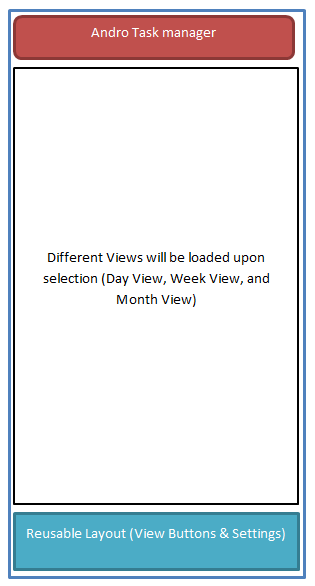
\includegraphics[scale=0.5]{hl.png}  &
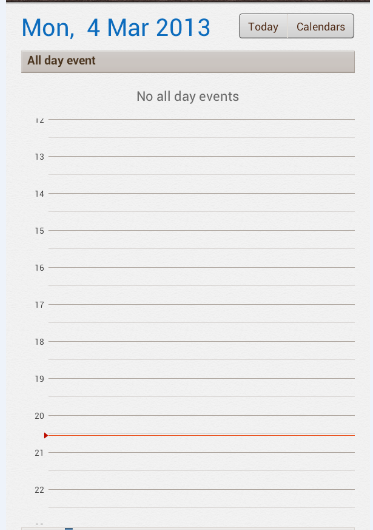
\includegraphics[scale=0.5]{day.png}
\end{array}$
\end{center}
\caption{High level view and Day view}
\label{abc}
\end{figure}

\begin{figure}[h!]
\begin{center}$
\begin{array}{cc}
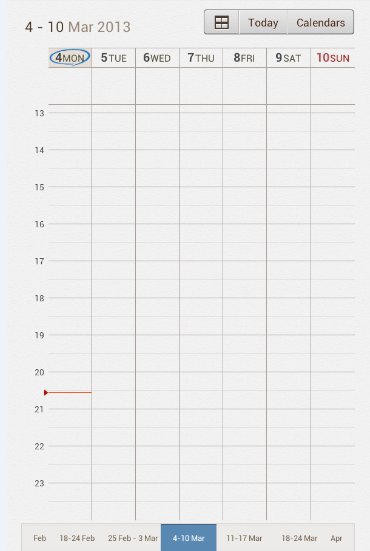
\includegraphics[scale=0.5]{week.png} &
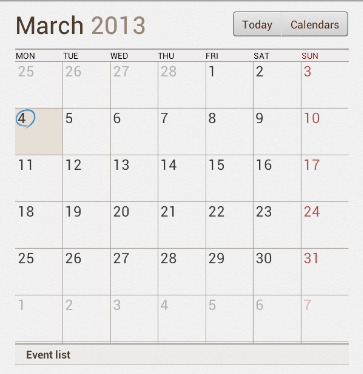
\includegraphics[scale=0.5]{month.png}
\end{array}$
\end{center}
\caption{Week and Month view UI}
\label{wm}
\end{figure}

\begin{figure}[h!]
\begin{center}
	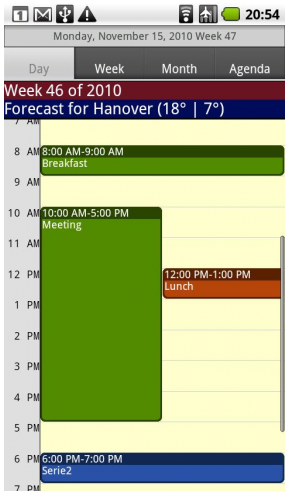
\includegraphics[scale=0.7, trim=125 0 50 0]{dvc.png}
	\caption{Scheduler Sample (Imaginary)}
\end{center}
\label{dvc}
\end{figure}



Figure~\ref{hd} provides the core fundamental UI for our project. Different view will be loaded upon user \texttt{"action"}. At the lower portion, it indicates \texttt{\textbf{Reusable layout}}  of Android feature. Android offers a variety of widgets to provide small and re-usable interactive elements to efficiently reuse complete layouts and embed another layout inside the current layout. Reusing layouts is particularly powerful as it allows you create reusable complex layouts that is expected for our desired project. It also will provide help for our application to extract commonalities across multiple layouts, managed separately. 

We ideate the week view and month view as like Figure~\ref{wm}. User can store their task in our app. Android provides several options to save persistent application data. As app data should be \texttt{private}, we can utilize \texttt{Shared Preferences} and \texttt{SQLite Storage}. Our app should not require that much storage. Figure~\ref{hd} represents an imaginary figure with user's stored tasks. UI will use \texttt{GridView}  or\texttt{Listview} displaying items in a two-dimensional, scrollable grid. The grid items are automatically inserted to the layout using a \texttt{ListAdapter}.

For testing purposes we use our own devices (Android smartphones), as this provides an easier and faster way to check the latest changes.

